\chapter{Lecteur de cartes}
Afin de vérifier l'assiduité des élèves lors des conférences nous mettons en
place un système de badge.

Il nous fallait un solution alliant plusieurs critères comme un coût et temps
de déceloppement réduit, fabilité.

\newpage

\section{Historique}
Dès le début du projet Monsieur Berry nous a proposé plusieurs pistes à 
explorer pour le badge en lui même. Il fallait que chaque participant aux
conférences puisse être identifié de manière unique:

\begin{itemize}
\item Money Kart: C'est une entreprise basée près de Grenoble, spécialisée
dans la création de cartes à puce, notament Moneo. L'avantage de cette solution
résidait dans la design des cartes des cartes. On aurait pû les faire graver
de façon à faire un buzz autour de la Semaine du Numérique. De plus la société
vendait également des lecteurs prêts à l'emploi.
Malheuresement, il nous fût impossible d'obtenir un devis pour de la part d'un
commercial, même après de multiples relance. Cette solution nécéssitait aussi
un investissement financier.

\item Carte étudiantes: Rapidement cette solution à fait l'unanimité. En effet,
elle était bien plus facile à mettre en place: chaque titulaire de carte délivrée
par l'UM2 possède un numéro unique, appelé numéro Mifare, accessible grâce à
la technologie RFID. Or Polytech possède une base de donnée faisant le lien entre
ce numéro et les élèves.
\end{itemize}

\section{RFID et Mifare}
RFID, de l'anglais ``radio frequency identification'' est une techonlogie 
mise au point pour permettre de lire à distance des données contenues dans des
marqueur, étiquette RFID.

    \begin{figure}[h]
        \begin{center}
            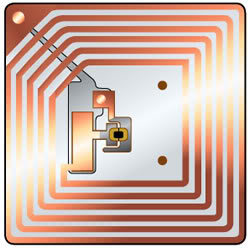
\includegraphics[scale=0.6]{RFIDtag.jpg} 
        \end{center}

        \caption{Etiquette RFID}
        \label{Etiquette RFID}
    \end{figure}


C'est une technologie employée quotidiennement par tout le monde puisqu'elle
sert entre autre à:

\begin{itemize}
\item Passeport bimométrique français.
\item Accès transport public, comme le tramay de Montpellier.
\item Inventaires.
\end{itemize}

Mifare est une des technologies de carte à puce sans contact les plus répandues
dans le monde avec 3,5 milliards de cartes et 40 millions de modules de lecture/encodage.

C'est deux technologies respectent des normes ISO.

\section{Cahier des charges}
\section{Modélisation}
\section{Recommandations}
